
\documentclass{article}
\usepackage[utf8]{inputenc}
\usepackage[utf8]{inputenc}
\usepackage{graphicx}
\usepackage{subcaption}
\usepackage{float}
\usepackage{amsmath}
\usepackage{amssymb}
\usepackage{enumerate}
\usepackage{physics}
\usepackage{siunitx}
\usepackage{tikz}
\usepackage{circuitikz}
\usepackage{indentfirst}

\usepackage{pgfplots}
\pgfplotsset{compat=1.18}

\addtolength{\oddsidemargin}{-.875in}
\addtolength{\evensidemargin}{-.875in}
\addtolength{\textwidth}{1.75in}

\addtolength{\topmargin}{-.875in}
\addtolength{\textheight}{1.75in} 
\title{HWtemplate}
\author{shomikchatterjee }
\date{April 2021}

\begin{document}
\begin{center}
\textbf{
{\Large ECE 210 Midterm 3 Worksheet}
}
\end{center} 
\noindent\makebox[\linewidth]{\rule{\linewidth}{0.4pt}}

\paragraph{Note:} This worksheet is not guaranteed to be entirely representative of the midterm's contents. Material may appear on this worksheet which will not appear on the midterm, and vice versa.

\subsection*{Partial Fraction Expansion}

\paragraph{1)} (Technique 1)

\subparagraph{a)} sub problem 1

\subparagraph{Solution} sub problem 1 solution

\[
sF(s) = s\frac{s+3}{s(s+2)(s+5)}=...
\]

\subparagraph{b)} sub problem 2

\subparagraph{Solution} sub problem 2 solution

\vfill

\paragraph{2)} (Technique 2)

\subparagraph{a)} sub problem 1

\subparagraph{Solution} sub problem 1 solution

\subparagraph{b)} sub problem 2

\subparagraph{Solution} sub problem 2 solution

\vfill

\newpage
\subsection*{S-Domain Circuit Analysis}

\paragraph{3)} In the circuit below, the switch has been open for a long time and is closed at $t=0$.
Let $I_A = 1~\text{mA}$, $L = 2~\text{H}$, $R = 1.5~\text{k}\Omega$, and $C = \frac{1}{6}~\mu\text{F}$.

\begin{figure}[ht!]
\centering
\begin{circuitikz}[american, transform shape]
  % current source (left branch)
  \draw (0,0) to[isource, l_=$I_A$] (0,4);
  % top and bottom rails
  \draw (0,4) -- (7.5,4);
  \draw (0,0) -- (7.5,0);
  % switch + inductor branch
  \draw (2,4) to[cspst, l={$t=0$}] (2,2.6);
  \draw (2,2.6) to[L, l_=$L$] (2,0);
  % resistor branch
  \draw (4,4) to[R, l_=$R$] (4,0);
  % capacitor branch
  \draw (6,4) to[C, l_=$C$] (6,0);
  % output voltage terminals
  \draw (6,4) to[short, -o] (7.5,4);
  \draw (6,0) to[short, -o] (7.5,0);
  \draw (7.5,4) to[open, v^=$v(t)$] (7.5,0);
  % junction dots
  \node[circ] at (2,4) {};
  \node[circ] at (4,4) {};
  \node[circ] at (6,4) {};
  \node[circ] at (2,0) {};
  \node[circ] at (4,0) {};
  \node[circ] at (6,0) {};
\end{circuitikz}
\end{figure}

\subparagraph{a)} Find the initial conditions $i_L(0^-)$ and $v(0^-)$, and draw the $s$-domain equivalent circuit for $t \geq 0$.

\subparagraph{Solution}
With the switch open for a long time, the circuit is in DC steady state. The inductor branch is disconnected, so $i_L(0^-) = 0$. The capacitor is fully charged, and acts as an open circuit, so all of $I_A$ flows through $R$:
\[
v(0^-) = R I_A = (1.5~\text{k}\Omega)(1~\text{mA}) = 1.5~\text{V}.
\]

For $t \ge 0$, the switch is closed, and we redraw the circuit in the $s$-domain using element transformations. Each energy-storage element becomes its impedance plus a source that accounts for its initial condition. Since all the elements share the same two nodes, we use the parallel (Norton) form for each:
\begin{itemize}
  \item \textbf{Current source:} $i_A(t) = I_A$ for $t \ge 0$, so it becomes $\dfrac{I_A}{s}$.
  \item \textbf{Resistor:} it is unchanged and stays $R$.
  \item \textbf{Inductor:} from $v_L(t) = L\,\dfrac{di_L}{dt}$ we get $V_L(s) = sL\,I_L(s) - L\,i_L(0)$, which gives $I_L(s) = \dfrac{V_L(s)}{sL} + \dfrac{i_L(0)}{s}$. This is an impedance $sL$ in parallel with a current source $\dfrac{i_L(0)}{s}$. Because $i_L(0^-) = 0$, this source is zero, and the inductor is just $sL$.
  \item \textbf{Capacitor:} from $i_C(t) = C\,\dfrac{dv_C}{dt}$ we get $I_C(s) = sC\,V_C(s) - C\,v_C(0)$. This is an impedance $\dfrac{1}{sC}$ in parallel with a current source $C\,v_C(0)$. Here $C\,v(0^-) = C\,(RI_A) = RCI_A$.
\end{itemize}
Putting these together, the $s$-domain circuit has $I_A/s$, $sL$, $R$, $1/sC$, and the capacitor's $RCI_A$ source all in parallel, with $V(s)$ across the output terminals. This is the circuit drawn below.


\begin{figure}[H]
\centering
\begin{circuitikz}[american, transform shape]
  % I_A/s source (left branch)
  \draw (0,0) to[isource, l_=$\frac{I_A}{s}$] (0,4);
  % top and bottom rails
  \draw (0,4) -- (10,4);
  \draw (0,0) -- (10,0);
  % sL branch
  \draw (2,4) to[L, l_=$sL$] (2,0);
  % R branch
  \draw (4,4) to[R, l_=$R$] (4,0);
  % 1/sC branch
  \draw (6,4) to[C, l_=$\frac{1}{sC}$] (6,0);
  % RCI_A initial-condition source
  \draw (8,0) to[isource, l=$RCI_A$] (8,4);
  % output terminals
  \draw (8,4) to[short, -o] (10,4);
  \draw (8,0) to[short, -o] (10,0);
  \draw (10,4) to[open, v^=$V(s)$] (10,0);
  % junction dots
  \foreach \x in {2,4,6,8}{
    \node[circ] at (\x,4) {};
    \node[circ] at (\x,0) {};
  }
\end{circuitikz}
\par\smallskip\textit{$s$-domain equivalent circuit for $t \ge 0$}
\end{figure}


\subparagraph{b)} 
Find the zero-state and zero-input components of $V(s)$, and then find $v_{zs}(t)$ and $v_{zi}(t)$ for $t \geq 0$.

\subparagraph{Solution} 
The equivalent impedance seen by both sources is the parallel combination of $sL$, $R$, and $1/sC$:
\[
Z_{eq}(s) = \left(\frac{1}{sL} + \frac{1}{R} + sC\right)^{-1}
= \frac{sLR}{s^2LRC + sL + R}
= \frac{s/C}{s^2 + \frac{1}{RC}s + \frac{1}{LC}}.
\]

\textbf{Zero-state} (only the $I_A/s$ source on):
\[
V_{zs}(s) = Z_{eq}(s)\,\frac{I_A}{s} = \frac{I_A/C}{s^2 + \frac{1}{RC}s + \frac{1}{LC}}.
\]

\textbf{Zero-input} (only the $RCI_A$ source on):
\[
V_{zi}(s) = Z_{eq}(s)\,RCI_A = \frac{R I_A\, s}{s^2 + \frac{1}{RC}s + \frac{1}{LC}}.
\]

\textbf{Substitute values.} Here $\frac{1}{RC} = 4000$, $\frac{1}{LC} = 3\times10^6$, $\frac{I_A}{C} = 6000$, and $RI_A = 1.5$. The denominator factors as
\[
s^2 + 4000s + 3\times 10^6 = (s+1000)(s+3000).
\]

Zero-state, by partial fractions:
\[
V_{zs}(s) = \frac{6000}{(s+1000)(s+3000)} = \frac{3}{s+1000} + \frac{-3}{s+3000}
\]
\[
\boxed{v_{zs}(t) = \left[3e^{-1000t} - 3e^{-3000t}\right]u(t)~\text{V}}
\]

Zero-input, by partial fractions:
\[
V_{zi}(s) = \frac{1.5\,s}{(s+1000)(s+3000)} = \frac{-0.75}{s+1000} + \frac{2.25}{s+3000}
\]
\[
\boxed{v_{zi}(t) = \left[-0.75e^{-1000t} + 2.25e^{-3000t}\right]u(t)~\text{V}}
\]


\vfill

\newpage

\subsection*{Marginal Stability \& Resonance}

\paragraph{4)} problem 1

\subparagraph{a)} marginal stability part

\subparagraph{Solution} sub problem 1 solution

\subparagraph{b)} resonance part

\subparagraph{Solution} sub problem 2 solution

\subparagraph{c)} etc

\subparagraph{Solution} sub problem 3 solution

\vfill

\paragraph{5)} problem 2

\subparagraph{a)} marginal stability part

\subparagraph{Solution} sub problem 1 solution

\subparagraph{b)} resonance part

\subparagraph{Solution} sub problem 2 solution

\subparagraph{c)} etc

\subparagraph{Solution} sub problem 3 solution

\vfill


\newpage

\subsection*{Fourier Transforms}

\paragraph{6)} Find the Fourier transform: $$g(t)=\frac{6}{t^2+9}$$

\subparagraph{Solution} This problem looks like the Fourier transform pair $$f(t)=e^{-a|t|}\longleftrightarrow F(\omega)=\frac{2a}{a^2+\omega^2}$$ with $a=3$. However, we have $f(t)$, not $F(\omega)$ matching the right-hand side.\\\\
To take care of this, we can use the Symmetry Property, which states that if $f(t)\longleftrightarrow F(\omega)$, then $$F(t)\longleftrightarrow2\pi f(-\omega)$$
Now, with $a=3$, we can evaluate: $f(-w)=e^{-3|-\omega|}=e^{-3|\omega|}$. Thus with the Symmetry Property, $$F(t)=\frac{2(3)}{3^2+t^2}=\frac{6}{t^2+9}\longleftrightarrow2\pi f(-\omega)=2\pi e^{-3|\omega|}$$
Finally, since $g(t)=F(t)$, we can conclude that the Fourier transform is $G(\omega)=2\pi e^{-|\omega|}$.

\newpage

\paragraph{7} Find the output: $$y(t)=e^{-2t}u(t)\ast \mathrm{rect}(\frac{t}{2})$$

\subparagraph{Solution} Let $h(t)=e^{-2t}u(t)$ and $f(t)=\mathrm{rect}(\frac{t}{2})$\\

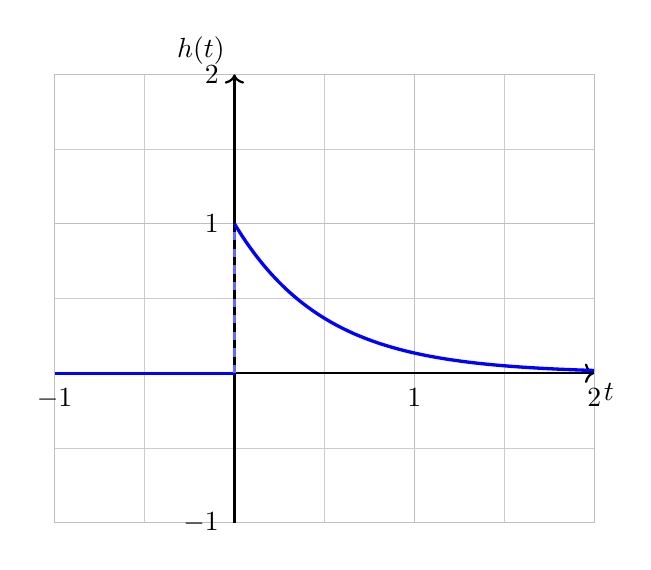
\begin{tikzpicture}
\begin{axis}[
    xmin=-1, xmax=2,
    ymin=-1, ymax=2,
    axis lines=middle,
    axis line style={->, thick},
    xlabel={\(t\)},
    ylabel={\(h(t)\)},
    xlabel style={anchor=north west},
    ylabel style={anchor=south east},
    grid=both,
    grid style={line width=0.2pt, draw=gray!30},
    major grid style={line width=0.4pt, draw=gray!50},
    grid style={line width=0.3pt, draw=gray!40},
    xminorgrids=true,
    yminorgrids=true,
    minor tick num=1,
    xtick={-1, 0, 1, 2},
    ytick={-1, 0, 1, 2},
    tick style={draw=none},
    samples=200
]

    \addplot[line width=1.2pt, blue, domain=-1:0] {0};
    \addplot[line width=1.2pt, blue, domain=0:2] {exp(-2*x)};

    \draw[dashed, blue!60, line width=0.8pt] (axis cs:0,0) -- (axis cs:0,1);

\end{axis}
\end{tikzpicture}
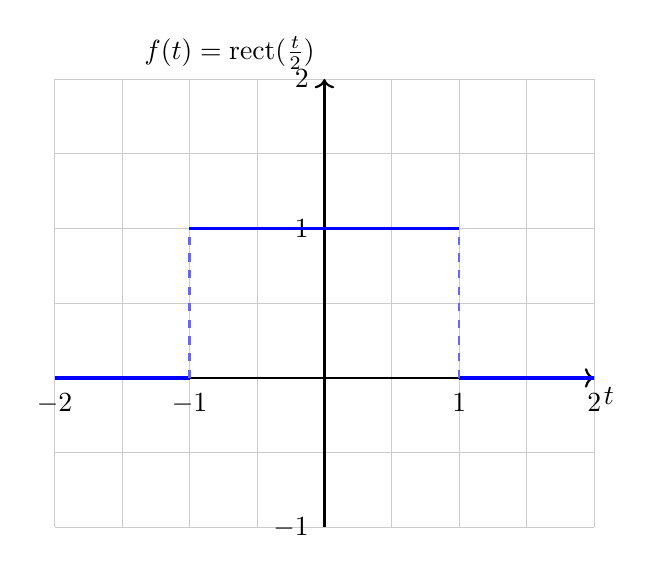
\begin{tikzpicture}
\begin{axis}[
    xmin=-2, xmax=2,
    ymin=-1, ymax=2,
    axis lines=middle,
    axis line style={->, thick},
    xlabel={\(t\)},
    ylabel={\(f(t)=\mathrm{rect}(\frac{t}{2})\)},
    xlabel style={anchor=north west},
    ylabel style={anchor=south east},
    grid=both,
    grid style={line width=0.3pt, draw=gray!40},
    xminorgrids=true,
    yminorgrids=true,
    minor tick num=1,
    xtick={-2, -1, 0, 1, 2},
    ytick={-1, 0, 1, 2},
    tick style={draw=none},
    samples=200
]

    \addplot[line width=1.2pt, blue, domain=-2:-1] {0};
    \addplot[line width=1.2pt, blue, domain=-1:1] {1};
    \addplot[line width=1.2pt, blue, domain=1:2] {0};

    \draw[dashed, blue!60, line width=0.8pt] (axis cs:-1,0) -- (axis cs:-1,1);
    \draw[dashed, blue!60, line width=0.8pt] (axis cs:1,0) -- (axis cs:1,1);

\end{axis}
\end{tikzpicture}

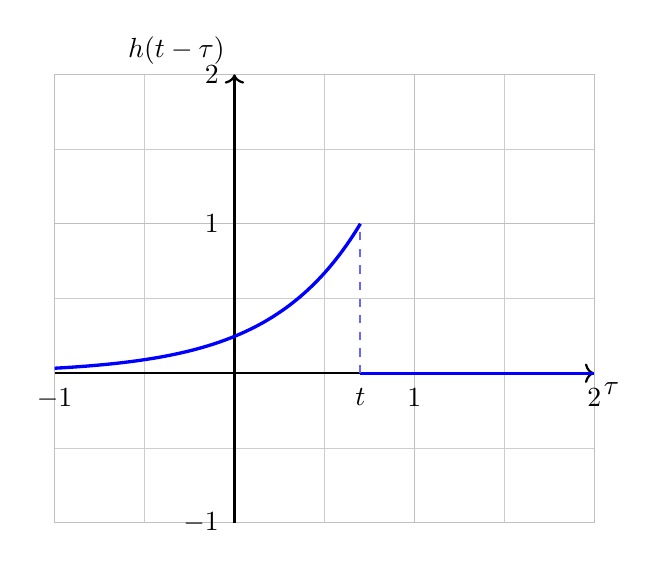
\begin{tikzpicture}
\begin{axis}[
    xmin=-1, xmax=2,
    ymin=-1, ymax=2,
    axis lines=middle,
    axis line style={->, thick},
    xlabel={\(\tau\)},
    ylabel={\(h(t-\tau)\)},
    xlabel style={anchor=north west},
    ylabel style={anchor=south east},
    grid=both,
    grid style={line width=0.2pt, draw=gray!30},
    major grid style={line width=0.4pt, draw=gray!50},
    grid style={line width=0.3pt, draw=gray!40},
    xminorgrids=true,
    yminorgrids=true,
    minor tick num=1,
    xtick={-1, 0, 1, 2},
    ytick={-1, 0, 1, 2},
    extra x ticks={0.7},
    extra x tick labels={\(t\)},
    extra x tick style={
        grid=none,
        tick label style={anchor=north}
    },
    tick style={draw=none},
    samples=200
]

    \addplot[line width=1.2pt, blue, domain=-1:0.7] {exp(-2*(0.7-x))};
    \addplot[line width=1.2pt, blue, domain=0.7:2] {0};

    \draw[dashed, blue!60, line width=0.8pt] (axis cs:0.7,0) -- (axis cs:0.7,1);
    
\end{axis}
\end{tikzpicture}

\begin{flalign*}
& y(t)=\int^{\infty}_{-\infty}h(t-\tau)f(\tau)\mathrm{d}\tau &&
\end{flalign*}\\
For $t<-1$: $y(t)=0$
For $-1\leq t<1$:
\[\begin{aligned}
y(t)&=\int^{t}_{-1}e^{-2(t-\tau)}\mathrm{d}\tau=e^{-2t}\int^{t}_{-1}e^{2\tau}\mathrm{d}\tau\\&=e^{-2t}\cdot\left[\frac{1}{2}e^{2\tau}\right]^{t}_{-1}=e^{-2t}\left[\frac{1}{2}e^{2t}-\frac{1}{2}e^{-2}\right]=\frac{1}{2}\left[1-e^{-2(t+1)}\right]
\end{aligned}\]
For $t\geq1$:
\[\begin{aligned}
y(t)&=\int^{1}_{-1}e^{-2(t-\tau)}\mathrm{d}\tau=e^{-2t}\int^{1}_{-1}e^{2\tau}\mathrm{d}\tau\\&=e^{-2t}\cdot\left[\frac{1}{2}e^{2\tau}\right]^{1}_{-1}=e^{-2t}\left[\frac{1}{2}e^{2}-\frac{1}{2}e^{-2}\right]=\frac{1}{2}(e^2-e^{-2})e^{-2t}
\end{aligned}\]
So,
\[\boxed{
y(t) = 
\begin{cases}
    0, & \text{if } t < -1 \\
    \frac{1}{2}\left[1-e^{-2(t+1)}\right], & \text{if } -1\leq t<1 \\
    \frac{1}{2}(e^2-e^{-2})e^{-2t},  & \text{if } t\geq1
\end{cases}
}\]
\vfill


\end{document}